\documentclass{article}
\usepackage{xeCJK}
\usepackage{amsmath}
\usepackage{listings}
\usepackage{xcolor}
\setlength{\parindent}{0pt}
\renewcommand{\baselinestretch}{1.0}
\lstset{
	frame=tb, % draw a frame at the top and bottom of the code block
	showstringspaces=false, % don't mark spaces in strings
	numbers=left, % display line numbers on the left
	commentstyle=\color{green}, % comment color
	keywordstyle=\color{blue}, % keyword color
	stringstyle=\color{red} % string color
}
\usepackage[a4paper,left=20mm,right=20mm,top=15mm,bottom=15mm]{geometry}  

\title{后缀数组}
\author{MengChunlei}

\begin{document}
\maketitle
\begin{itemize}
	\item 定义
	\item 一般做法
	\item 改进做法
	\item 计数排序
	\item 基数排序
	\item 最后的改进
	\item 一些优化
	\item height数组
	\item 应用
\end{itemize}
\section{定义}
对于一个长度为$n$的字符串$s:s[0],s[1],...,s[n-2],s[n-1]$,它对应的后缀数组也是一个长度为$n$的数组$sa$.其中$sa[i]$表示在所有$n$个后缀中,排第$i$名的后缀是哪个(第一个字母在$s$中的位置).
比如$s$=aabaaaab,那么对应的$sa$ 为: \par
$\begin{matrix} 
index & 0 & 1 & 2 & 3 & 4 & 5 & 6 & 7 \\ 
s & a & a & b & a & a & a & a & b \\ 
sa & 3 & 4 & 5 & 0 & 6 & 1 & 7 & 2 \\
\end{matrix}$ \par
第0名: aaaab\par
第1名: aaab\par
第2名: aab\par
第3名: aabaaaab\par
第4名: ab\par
第5名: abaaaab\par
第6名: b\par
第7名: baaaab\par
另外还有一个数组称之为rank数组$rk$,它的长度也是$n$,$rk[i]$表示以$s[i]$开始的后缀的排名.那么有以下关系: \par
$sa[rk[i]]=rk[sa[i]]=i$ \par
\section{一般做法}
很容易想到$n^{2}log(n)$的做法.代码如下: \par
\begin{lstlisting}[language=C++, caption={Normal}]
std::vector<int> ComputeSA1(const std::string &s) {
  int n = static_cast<int>(s.size());
  std::vector<int> sa(n);
  for (int i = 0; i < n; ++i) {
    sa[i] = i;
  }
  std::sort(sa.begin(), sa.end(), [&](int p1, int p2) {
    for (; p1 < n && p2 < n && s[p1] == s[p2]; ++p1, ++p2);
    return p1 < n && p2 < n ? s[p1] < s[p2] : p1 == n;
  });
  return sa;
}
\end{lstlisting}

\section{改进做法}
优化的思路是这样的:设$rk_{w}[i]$表示以$i$开始的长度为$w$的子串的排名,即$s[i]\rightarrow s[i+w-1]$.那么对于$rk_{2w}$来说,它的计算可以借助于$rk_{w}$来进行.简答来说, 就是以$rk_{w}[i]$为第一关键字,以$rk_{w}[i+w]$为第二关键字进行排序,就可以求出$rk_{2w}$数组.
\begin{lstlisting}[language=C++, caption={Better}]
std::vector<int> UpdateRank(const std::vector<int> &sa,
  const std::vector<int> &old_rank, int n, int w) {
  std::vector<int> rk(n);
  rk[sa[0]] = 0;
  for (int p = 0, i = 1; i < n; ++i) {
    if (old_rank[sa[i]] == old_rank[sa[i - 1]] &&
       ((sa[i] + w >= n && sa[i - 1] + w >= n) ||
        (sa[i] + w < n && sa[i - 1] + w < n &&
         old_rank[sa[i] + w] == old_rank[sa[i - 1] + w]))) {
      rk[sa[i]] = p;
    } else {
      rk[sa[i]] = ++p;
    }
  }
  return rk;
}
std::vector<int> ComputeSA2(const std::string &s) {
  int n = static_cast<int>(s.size());
  std::vector<int> sa(n);
  std::vector<int> rk(n);
  for (int i = 0; i < n; ++i) {
    sa[i] = i;
    rk[i] = s[i];
  }
  for (int w = 1; w < n; w <<= 1) {
    std::sort(sa.begin(), sa.end(), [&](int x, int y) {
      return rk[x] == rk[y]
                 ? (x + w < n && y + w < n ? rk[x + w] < rk[y + w] : x + w >= n)
                 : rk[x] < rk[y];
    });
    rk = UpdateRank(sa, rk, n, w);
  }
  return sa;
}
\end{lstlisting}
这个算法的复杂度为$O(nlog^{2}(n))$.接下来,进一步的改进需要借助于计数排序和基数排序.先了解下.

\section{计数排序}
假设一个待排列的序列中所有的元素只有$C$种, 那么可以通过计算每种元素的个数进行排列. 假设排列的元素有$n$个.这个的复杂度为$O(n+C)$. 示例代码如下: \par
\begin{lstlisting}[language=C++, caption={Counting Sort}]
template <typename Elem>
std::vector<Elem> CountingSort(const std::vector<Elem> &eles,
                               std::function<int(const Elem &)> functor,
                               int C) {
  int n = static_cast<int>(eles.size());
  std::vector<int> bucket(C, 0);
  for (int i = 0; i < n; ++i) {
    ++bucket[functor(eles[i])];
  }
  for (int i = 1; i < C; ++i) {
    bucket[i] += bucket[i - 1];
  }
  std::vector<Elem> result(n);
  for (int i = n - 1; i >= 0; --i) {
    result[--bucket[functor(eles[i])]] = eles[i];
  }
  return result;
}
\end{lstlisting}
由14-16行可以看出, 这是一个稳定排序算法.

\section{基数排序}
如果待排序的元素有$k$个关键字, 可以先对第$k$个关键字进行稳定排序, 然后再对第$k-1$个元素进行稳定排序,以此类推,最后对第$1$个关键字进行稳定排序.如下图所示: \par
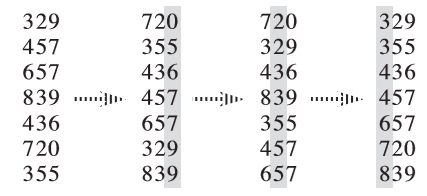
\includegraphics[scale=0.6]{pic1.png} \par
下面是代码示例: \par
\begin{lstlisting}[language=C++, caption={Radix Sort}]
template <typename Elem>
std::vector<Elem>
RadixSort(const std::vector<Elem> &eles, int k, const std::vector<int> &cs,
          std::function<int(const Elem &, int index)> functor) {
  std::vector<Elem> result = eles;
  for (int i = k - 1; i >= 0; --i) {
  result = CountingSort<Elem>(
      result, std::bind(functor, std::placeholders::_1, i), cs[i]);
  }
  return result;
}

\end{lstlisting}

\section{最后的改进}
对第三步中$nlog^{2}(n)$的方法进行进行改进.可以将循环内的每次排序看作是两个关键字的排序,先对第二个关键字排序, 再对第一个关键字排序. \par
\begin{lstlisting}[language=C++, caption={Last Improvement}]
std::vector<int> ComputeSA3(const std::string &s) {
  int n = static_cast<int>(s.size());
  int m = std::max(256, n) + 1;
  std::vector<int> sa(n);
  std::vector<int> rk(n);
  std::vector<int> cnt(m, 0);
  for (int i = 0; i < n; ++i) {
    ++cnt[rk[i] = s[i]];
  }
  for (int i = 1; i < m; ++i) {
    cnt[i] += cnt[i - 1];
  }
  for (int i = n - 1; i >= 0; --i) {
    sa[--cnt[rk[i]]] = i;
  }
  for (int w = 1; w < n; w <<= 1) {
    sa = RadixSort<int>(sa, 2, {m, m}, [&](const int &x, int index) {
      if (index == 0) {
        return rk[x];
      } else {
        return x + w >= n ? 0 : rk[x + w] + 1;
      }
    });
    rk = UpdateRank(sa, rk, n, w);
  }
  return sa;
}
\end{lstlisting}
这个算法的复杂度为 $O(nlog(n))$
\end{document}
